\chapter{Biodiversidade}\label{ch:g5:biodiversity}

Pegue um metro quadrado de campo florido e comece a contar: uma
dúzia de tipos de \omterm{def:g1:plants-around-us:plant}{plantas}, besouros e percevejos sem conta, aranhas,
caracóis, minhocas embaixo e borboletas em cima. Agora tente o mesmo
metro quadrado de pátio de escola calçado. A diferença entre essas
duas contagens tem um nome --- \omterm{def:g5:biodiversity:biodiversity}{biodiversidade} --- e virou uma das
palavras mais importantes da \omterm{def:g1:living-or-not:living}{biologia}.

\section{A diversidade da vida}

\begin{definition}[Espécie]\label{def:g5:biodiversity:species}
Uma \emph{espécie}\index{espécie} é um tipo específico de \omterm{def:g1:living-or-not:living}{ser vivo}:
todos os indivíduos construídos no mesmo modelo, que se reproduzem
entre si. O pardal é uma espécie; a margarida comum também, e a
raposa-vermelha, e o caracol de jardim. As classes do
\cref{ch:g4:classifying-animals} são caixas com muitas espécies:
``\omterm{prop:g3:sorting-living-things:groups}{mamíferos}'' guarda milhares delas.
\end{definition}

\begin{definition}[Biodiversidade]\label{def:g5:biodiversity:biodiversity}
A \emph{biodiversidade}\index{biodiversidade} de um lugar é a
variedade de vida que ele abriga --- acima de tudo, quantas
\emph{\omterm{def:g5:biodiversity:species}{espécies}} diferentes vivem ali e como cada uma delas está
indo. Um campo florido, rico em \omterm{def:g5:biodiversity:species}{espécies}, tem biodiversidade alta;
um pátio calçado, quase nenhuma.
\end{definition}

\begin{omfigure}
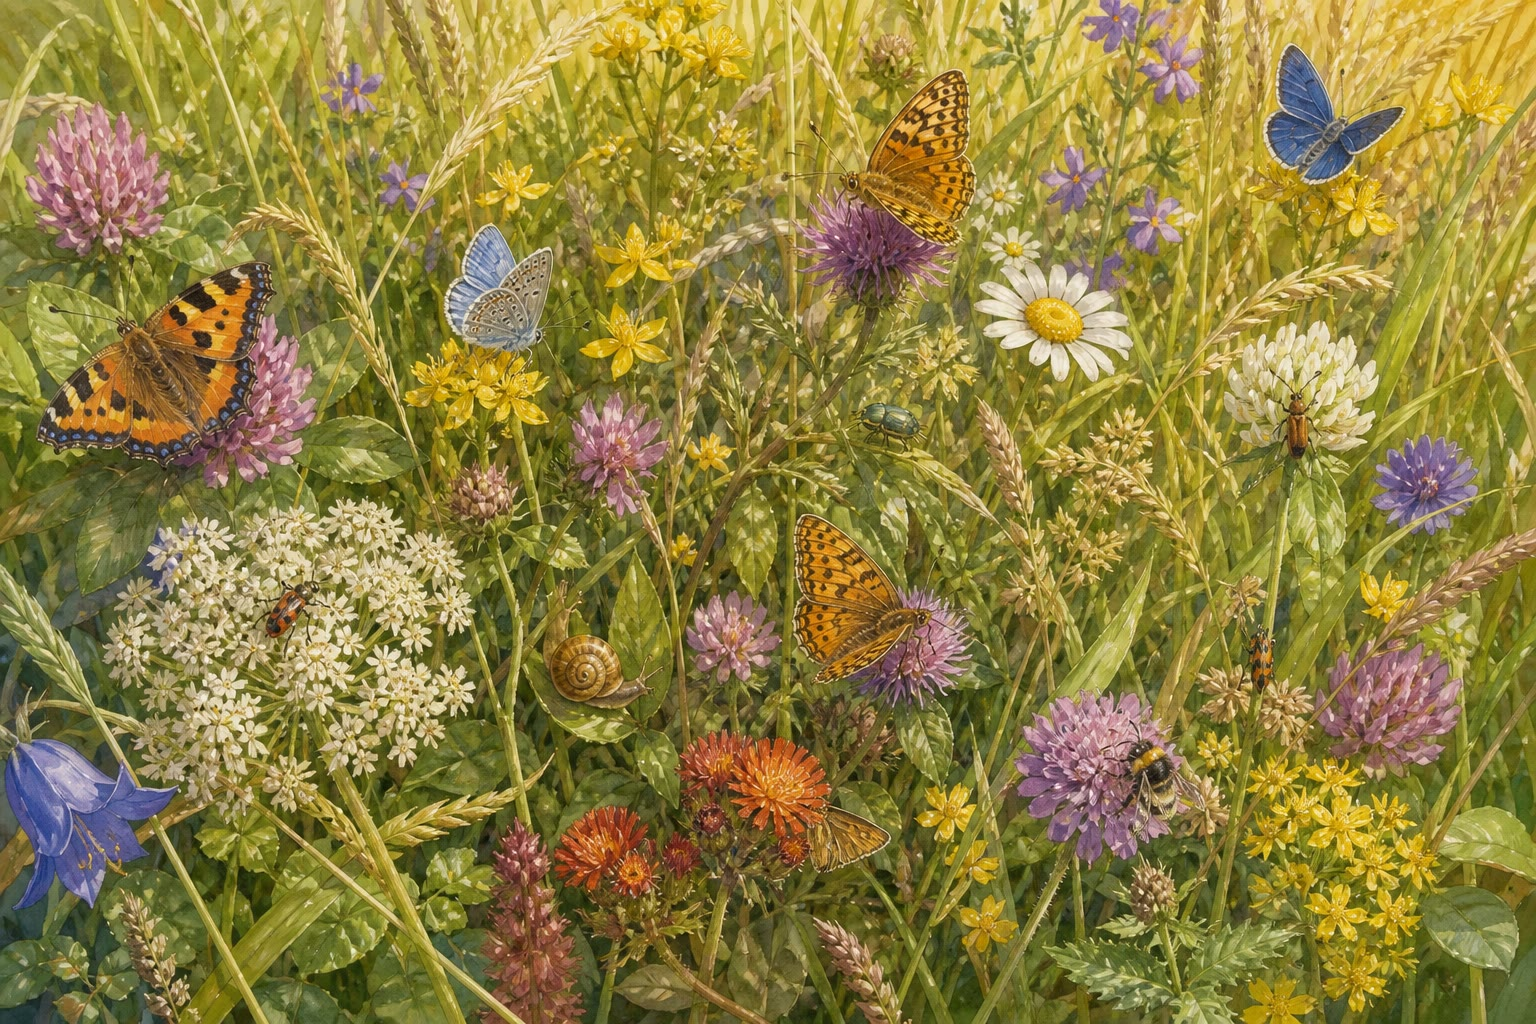
\includegraphics[width=0.62\linewidth]{images/book1/ai/g5-biodiversity-meadow.jpg}

{\small Um metro quadrado de campo, no meio da contagem: gramíneas,
\omterm{def:g3:flowers-fruits-seeds:parts}{flores}, borboletas, besouros, um caracol --- e a contagem mal
começou.}
\end{omfigure}

\begin{example}[Contando o planeta]\label{ex:g5:biodiversity:planet}
Os cientistas já nomearam cerca de dois milhões de \omterm{def:g5:biodiversity:species}{espécies} --- e
têm certeza de que isso é só uma parte do total, porque \omterm{def:g5:biodiversity:species}{espécies}
novas aparecem em toda expedição séria: besouros acima de tudo
(nenhum grupo tem mais \omterm{def:g5:biodiversity:species}{espécies} nomeadas), mas também \omterm{prop:g3:sorting-living-things:groups}{peixes}, sapos,
\omterm{def:g1:plants-around-us:plant}{plantas} e até \omterm{prop:g3:sorting-living-things:groups}{mamíferos} de vez em quando. A contagem completa de
\omterm{def:g5:biodiversity:species}{espécies} da Terra ainda é desconhecida --- quase todas as
estimativas chegam a milhões além do que já foi nomeado.
\end{example}

\begin{remark}[Diversidade em todas as escalas]\label{rem:g5:biodiversity:scales}
A \omterm{def:g5:biodiversity:biodiversity}{biodiversidade} aparece em várias escalas ao mesmo tempo: muitas
\omterm{def:g5:biodiversity:species}{espécies} num \omterm{def:g2:where-animals-live:habitat}{hábitat}; muitos \omterm{def:g2:where-animals-live:habitat}{hábitats} diferentes lado a lado (lagoa,
cerca viva, campo --- cada um com as \omterm{def:g5:biodiversity:species}{espécies} dele, como mostrou o
\cref{ex:g2:where-animals-live:four}); e, dentro de uma \omterm{def:g5:biodiversity:species}{espécie}, dois
indivíduos nunca são exatamente iguais --- dois caracóis de jardim
nunca usam a mesma \omterm{def:g1:animals-around-us:covering}{concha}. Variedade dentro de variedade dentro de
variedade.
\end{remark}

\section{Por que a biodiversidade importa}

\begin{proposition}[A teia precisa dos fios dela]\label{prop:g5:biodiversity:web}
As \omterm{def:g5:biodiversity:species}{espécies} de um \omterm{def:g2:where-animals-live:habitat}{hábitat} se alimentam, se abrigam, se polinizam e
se limpam umas às outras --- elas são fios de uma mesma teia
(\cref{rem:g3:food-chains:web}). Uma teia rica, com muitos fios,
consegue absorver um baque: se uma \omterm{def:g5:biodiversity:species}{espécie} de presa falha, os
caçadores dela mudam para outras. Uma teia pobre rasga fácil: cada
\omterm{def:g5:biodiversity:species}{espécie} perdida deixa as sobreviventes com menos opções. A
\omterm{def:g5:biodiversity:biodiversity}{biodiversidade} é a força da teia.
\end{proposition}
\admitted

\begin{example}[O teste do pomar]\label{ex:g5:biodiversity:orchard}
Um pomar com cercas vivas, faixas de \omterm{def:g3:flowers-fruits-seeds:parts}{flores} silvestres e árvores
velhas abriga dezenas de \omterm{def:g5:biodiversity:species}{espécies} ajudantes: abelhas e moscas-das-flores
polinizam as \omterm{def:g3:flowers-fruits-seeds:parts}{flores}
(\cref{rem:g3:flowers-fruits-seeds:bees}), joaninhas comem os
pulgões, \omterm{prop:g3:sorting-living-things:groups}{aves} patrulham atrás de \omterm{ex:g2:animals-grow-up:butterfly}{lagartas}, minhocas mantêm a terra
arejada. Arranque as cercas vivas e corte as \omterm{def:g3:flowers-fruits-seeds:parts}{flores}, e os ajudantes
vão embora --- quem cultiva a fruta passa então a fazer sozinho os
trabalhos deles, trabalhos que a teia fazia de graça.
\end{example}

\begin{example}[As pessoas vivem da teia]\label{ex:g5:biodiversity:people}
Tudo o que os seres humanos comem remonta a \omterm{def:g5:biodiversity:species}{espécies} vivas
(\cref{rem:g4:what-plants-need:everyone}); quase todos os nossos
remédios foram encontrados primeiro em \omterm{def:g1:plants-around-us:plant}{plantas}, mofos e outros \omterm{def:g1:living-or-not:living}{seres
vivos}; algodão, lã, madeira e couro são produtos de \omterm{def:g5:biodiversity:species}{espécies}. Os
fios da teia passam direto por toda cozinha, farmácia e guarda-roupa.
\end{example}

\section{A biodiversidade pode se perder --- e ser ajudada}

\begin{proposition}[Como a diversidade se perde]\label{prop:g5:biodiversity:loss}
Uma \omterm{def:g5:biodiversity:species}{espécie} diminui quando lhe tiram aquilo de que ela depende:
\begin{itemize}
  \item o \emph{\omterm{def:g2:where-animals-live:habitat}{hábitat}} destruído --- a lagoa aterrada da
        \cref{prop:g2:where-animals-live:loss}, a cerca viva
        arrancada, o campo calçado;
  \item o \omterm{def:g2:caring-for-nature:environment}{ambiente} envenenado --- lixo e produtos químicos
        (\cref{prop:g2:caring-for-nature:harm});
  \item indivíduos demais retirados --- pesca, colheita ou caça em
        excesso.
\end{itemize}
Uma \omterm{def:g5:biodiversity:species}{espécie} totalmente sumida --- em toda parte, para sempre --- está
\emph{extinta}\index{extinto}. A extinção não é como um jogo perdido:
não existe rodada seguinte.
\end{proposition}
\admitted

\begin{method}[Ajudar a biodiversidade, começando pequeno]\label{met:g5:biodiversity:help}
As receitas do \cref{met:g2:caring-for-nature:rules} funcionam também
em escala maior:
\begin{enumerate}
  \item guarde e plante variedade --- uma cerca viva de cinco
        arbustos ganha de um muro, uma faixa de \omterm{def:g3:flowers-fruits-seeds:parts}{flores} ganha do
        cascalho pelado;
  \item deixe cantos selvagens: madeira morta, pilhas de \omterm{def:g1:plants-around-us:parts}{folhas} e
        grama sem corte são \omterm{def:g2:where-animals-live:habitat}{hábitats}
        (\cref{ex:g2:caring-for-nature:home});
  \item ajude os ajudantes: caixas de ninho, abrigos para \omterm{prop:g3:sorting-living-things:groups}{insetos},
        uma lagoa por menor que seja
        (\cref{ex:g2:where-animals-live:schoolpond});
  \item conte o que vive em volta de você, ano após ano --- o que é
        contado é notado, e o que é notado acaba protegido.
\end{enumerate}
\end{method}

\begin{example}[A volta das cegonhas]\label{ex:g5:biodiversity:storks}
Onde campos alagados foram restaurados e plataformas de ninho foram
erguidas, as cegonhas --- que já tinham quase sumido de regiões
inteiras --- voltaram a se reproduzir, e com elas voltaram sapos,
libélulas e \omterm{def:g3:flowers-fruits-seeds:parts}{flores} de campo. As \omterm{def:g5:biodiversity:species}{espécies} voltam quando os fios delas
são reatados: a proteção funciona, e os resultados dela podem ser
observados da praça da cidade.
\end{example}

\section{Exercícios}

\begin{exercise}[$\star$]\label{exo:g5:biodiversity:1}
O que é uma \omterm{def:g5:biodiversity:species}{espécie}? Dê três exemplos deste capítulo.
\end{exercise}

\begin{exercise}[$\star$]\label{exo:g5:biodiversity:2}
O que é \omterm{def:g5:biodiversity:biodiversity}{biodiversidade}? Compare o campo e o pátio calçado.
\end{exercise}

\begin{exercise}[$\star$]\label{exo:g5:biodiversity:3}
Mais ou menos quantas \omterm{def:g5:biodiversity:species}{espécies} já foram nomeadas? Por que o número
verdadeiro é certamente maior?
\end{exercise}

\begin{exercise}[$\star$]\label{exo:g5:biodiversity:4}
Diga as três escalas de diversidade da
\cref{rem:g5:biodiversity:scales}, cada uma com o exemplo dela.
\end{exercise}

\begin{exercise}[$\star$]\label{exo:g5:biodiversity:5}
Por que uma teia rica em \omterm{def:g5:biodiversity:species}{espécies} sobrevive melhor aos baques do que
uma teia pobre? Use o argumento dos caçadores que trocam de presa.
\end{exercise}

\begin{exercise}[$\star$]\label{exo:g5:biodiversity:6}
Liste quatro \omterm{def:g5:biodiversity:species}{espécies} ajudantes do pomar e o trabalho gratuito que
cada uma faz.
\end{exercise}

\begin{exercise}[$\star$]\label{exo:g5:biodiversity:7}
Dê os três jeitos de uma \omterm{def:g5:biodiversity:species}{espécie} diminuir, com um exemplo de cada. O
que quer dizer \emph{\omterm{prop:g5:biodiversity:loss}{extinta}}?
\end{exercise}

\begin{exercise}[$\star$]\label{exo:g5:biodiversity:8}
Faça a experiência: conte as \omterm{def:g5:biodiversity:species}{espécies} --- \omterm{def:g1:plants-around-us:plant}{plantas} e \omterm{def:g1:animals-around-us:animal}{animais},
nomeados ou descritos --- num quadradinho que você escolher lá fora.
Depois conte um quadradinho calçado, para comparar. Os seus dois
números são uma medição de \omterm{def:g5:biodiversity:biodiversity}{biodiversidade}.
\end{exercise}

\begin{exercise}[$\star\star$]\label{exo:g5:biodiversity:9}
``Perder uma \omterm{def:g5:biodiversity:species}{espécie} de besouro entre milhares não pode fazer
diferença.'' Responda com a \cref{prop:g5:biodiversity:web} --- e com
o fato de que ninguém conhece todos os fios que uma \omterm{def:g5:biodiversity:species}{espécie} segura.
\end{exercise}

\begin{exercise}[$\star\star$]\label{exo:g5:biodiversity:10}
A história das cegonhas é chamada de sucesso da proteção do
\emph{\omterm{def:g2:where-animals-live:habitat}{hábitat}}, e não da proteção das cegonhas uma a uma. Explique a
diferença, usando a \cref{prop:g2:where-animals-live:loss} e o que
voltou junto com as cegonhas.
\end{exercise}

\begin{exercise}[$\star\star\star$]\label{exo:g5:biodiversity:11}
Quem cuida de um pomar troca as cercas vivas e as faixas de \omterm{def:g3:flowers-fruits-seeds:parts}{flores}
por muros e cascalho, e depois precisa alugar colmeias para a
polinização e pulverizar contra os pulgões --- gastando dinheiro com
trabalhos que antes eram feitos de graça. Use o
\cref{ex:g5:biodiversity:orchard} para explicar o que foi retirado
de verdade --- e por que as contas do trabalho gratuito da natureza
quase sempre só aparecem depois que ele para.
\end{exercise}
